\documentclass[class=article,border=5pt,tikz]{standalone}
\usetikzlibrary{shapes.geometric}

\begin{document}
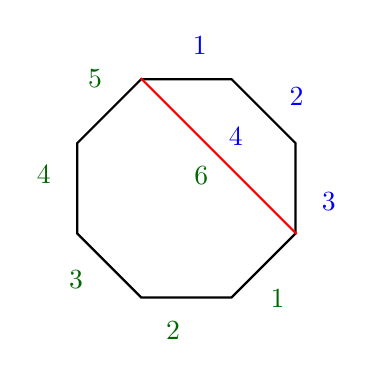
\begin{tikzpicture}[thick,x=1cm,y=1cm]
   \node [regular polygon,regular polygon sides=8,draw,minimum width=3cm]
   (octagon){};
   % define coordinates for the diagonal
   \coordinate (A) at (octagon.corner 7);
   \coordinate (B) at (octagon.corner 2);
   % draw the diagonal
   \draw [red]  (A) -- (B); 
   % draw the 6 sides on one side of the division
   \foreach [evaluate=\x as \y using int(6-\x)] \x in {1,...,5} {
       \pgfmathtruncatemacro{\xx}{\x+1}
       \path (octagon.corner \x)--(octagon.corner \xx) node [green!40!black,pos=1.5] {\y};}
   % manually add label to the diagonal
   \path (A) -- (B) node [midway,below left,green!40!black] {6};
   % draw the 4 sides on the other side of the division
   \foreach [evaluate=\x as \y using int(9-\x)] \x in {6,...,8} {
       \pgfmathtruncatemacro{\xx}{Mod(\x,8)+1}
       \path (octagon.corner \x)--(octagon.corner \xx) node [blue,pos=1.5] {\y};}
   % manually add label to the diagonal
   \path (A) -- (B) node [midway,above right,blue] {4};
\end{tikzpicture}
\end{document}

       %\node [above, minimum size=6mm] at (octagon.corner \x) {\y};